\section{Integral Theorems}
\subsection{Green's theorem}
\begin{theorem}[Green]\label{thm:Green}
    If $P = P(x, y)$ and $Q = Q(x, y)$ are continuously differentiable functions on $A \cup \partial A$ and $\partial A$ is \textit{piecewise smooth}, then
    \[
        \oint_{\partial A} P \mathrm{~d} x+Q \mathrm{~d} y=\iint_{A}\left(\frac{\partial Q}{\partial x}-\frac{\partial P}{\partial y}\right) \mathrm{d} x \mathrm{~d} y.
    \]
    Orientation of $ \partial A $ is such that $A$ lies to your left as you traverse it.
\end{theorem}
\begin{center}
    \begin{tikzpicture}
        \filldraw [color=black, thick, fill=black!20, arrow inside={end=latex',opt={black,scale=1.6}}{0,0.25,0.5,0.75}] (0,0) circle (1.5);
        \filldraw [color=black, thick, fill=white,<-] (0,0) circle (0.75);
    \end{tikzpicture}
\end{center}
\begin{note}
    It is easy to establish the result for a rectangle. Let 
    \[
        A = \{(x,y):a\le x\le b,c\le y\le d\}.
    \]
    In this case, RHS is 
    \begin{align*}
        &\int_{c}^{d} \int_{a}^{b} \frac{\partial Q}{\partial x}  \,\mathrm{d}x \,\mathrm{d}y-\int_{a}^{b} \int_{c}^{d} \frac{\partial P}{\partial y}  \,\mathrm{d}y \,\mathrm{d}x\\ 
        =& \int_{c}^{d} Q(b,y)-Q(a,y) \,\mathrm{d}y+\int_{a}^{b} P(x,c)-P(x,d) \,\mathrm{d}x\\ 
        =& \oint_{\partial A} P\dd x+Q\dd y.
    \end{align*}
    \begin{center}
        \begin{tikzpicture}
            \fill [black!20] (-2, -1) rectangle (1, 1);
            \node at (-0.5, 0) {$A$};
            \node [below] at (-1, -2) {$\dd y=0,y=c$};
            \node [above] at (0, 2) {$\dd y=0,y=d$};
            \node [right] at (2,0.5) {$ \dd x=0,x=b$};
            \node [left] at (-3,-0.5) {$ \dd x=0,x=b$};
            \draw [->-=0.5,thick] (-2, -1) -- (1, -1);
            \draw [->-=0.5,thick] (1, -1) -- (1, 1);
            \draw [->-=0.5,thick] (1, 1) -- (-2, 1);
            \draw [->-=0.5,thick] (-2, 1) -- (-2, -1);
            \draw [->] (0, 2) -- (0, 1) ;
            \draw [->] (-1, -2) -- (-1, -1);
            \draw [->] (2,0.5) -- (1,0.5);
            \draw [->] (-3,-0.5) -- (-2,-0.5);
        \end{tikzpicture}
    \end{center}
\end{note}
\begin{example}
    Let $(P, Q)=\left(-\frac{1}{2} y, \frac{1}{2} x\right) .$ Then Green's theorem tells us
    \[
    \operatorname{area}(A)=\iint_{A} \mathrm{~d} x \mathrm{~d} y=\frac{1}{2} \oint_{\partial A} x \mathrm{~d} y-y \mathrm{~d} x
    \]
    Let $A$ be the ellipse $x^{2} / a^{2}+y^{2} / b^{2} \leq 1$ so that $\partial A$ has parametrisation
    \[
    [0,2 \pi] \ni t \mapsto \begin{pmatrix}
        a \cos t \\
        b \sin t
    \end{pmatrix}
    \]
    Then
    \[
    \operatorname{area}(A)=\frac{1}{2} \int_{0}^{2 \pi}\left(a b \cos ^{2} t+a b \sin ^{2} t\right) \mathrm{d} t=\pi a b,
    \]
    as expected.
\end{example}

\subsection{Stokes' Theorem}
\begin{theorem}[Stokes]\label{thm:Stokes}
    If $ \bfF = \bfF(\bfx) $ is a continuously differentiable vector field and $S$ is an orientable piecewise regular surface with piecewise smooth boundary $ \partial  S $, then 
    \[
        \int_{S} (\curl\bfF) \cdot\mathrm{d}\mathbf{S} = \oint_{\partial S} \bfF \cdot\mathrm{d}\mathbf{x}
    \]
\end{theorem}
\begin{note}
    The ``orientable'' bit means there is a \textit{consistent} choice of normal vector at each point of $S$. i.e. $S$ has two sides. e.g. \mobius band is not orientable.
    \begin{center}
    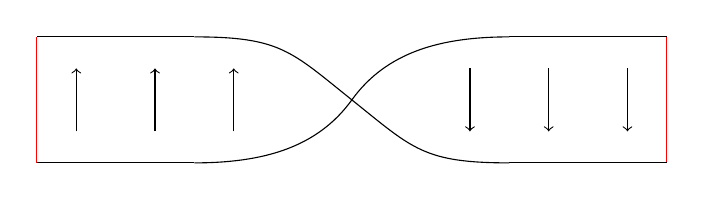
\begin{tikzpicture}[yscale=0.8]
        \node (0) at (-4, 3) {};
        \node (1) at (-4, 1) {};
        \node (2) at (4, 3) {};
        \node (3) at (4, 1) {};
        \node (4) at (2, 3) {};
        \node (5) at (2, 1) {};
        \node (6) at (-2, 3) {};
        \node (7) at (-2, 1) {};
        \node (8) at (0, 2) {};
        \node (9) at (-4, 3) {};
        \node (10) at (-3.5, 1.5) {};
        \node (11) at (-3.5, 2.5) {};
        \node (12) at (-2.5, 1.5) {};
        \node (13) at (-2.5, 2.5) {};
        \node (14) at (-1.5, 1.5) {};
        \node (15) at (-1.5, 2.5) {};
        \node (16) at (1.5, 2.5) {};
        \node (17) at (1.5, 1.5) {};
        \node (18) at (2.5, 2.5) {};
        \node (19) at (2.5, 1.5) {};
        \node (20) at (3.5, 2.5) {};
        \node (21) at (3.5, 1.5) {};
        \node (22) at (3.5, 1.5) {};
        \draw [red] (1.center) to (9.center);
        \draw (9.center) to (6.center);
        \draw [in=135, out=0, looseness=1.25] (6.center) to (8.center);
        \draw [in=-180, out=60] (8.center) to (4.center);
        \draw (4.center) to (2.center);
        \draw [red] (2.center) to (3.center);
        \draw (3.center) to (5.center);
        \draw [in=-45, out=-180, looseness=1.25] (5.center) to (8.center);
        \draw [in=0, out=-120] (8.center) to (7.center);
        \draw (7.center) to (1.center);
        \draw [->] (20.center) to (22.center);
        \draw [->] (18.center) to (19.center);
        \draw [->] (16.center) to (17.center);
        \draw [->] (14.center) to (15.center);
        \draw [->] (12.center) to (13.center);
        \draw [->] (10.center) to (11.center);
    \end{tikzpicture}\\
    \begin{tikzpicture}[scale=1.25]
        \begin{axis}
          [
            hide axis,
            view={40}{40}
          ]
          \addplot3
          [
            mesh, shader=faceted interp,
            point meta=x,
            colormap/blackwhite,
            samples=100,
            samples y=5,
            z buffer=sort,
            domain=0:360,
            y domain=-0.5:0.5,
          ]
          (%
            {(1+0.5*y*cos(x/2)))*cos(x)},
            {(1+0.5*y*cos(x/2)))*sin(x)},
            {0.5*y*sin(x/2)}
          );
          \addplot3
          [
            samples=50,
            domain=-145:180,
            samples y=0,
            thick,
            postaction={decorate},
            decoration={% pgfplots manual 355-356
              markings,
              mark=between positions 0 and 1 step 2.5mm with
              {
                \node [single arrow, transform shape, rotate=-90, fill, draw, inner sep=0pt, single arrow head extend=1pt, text width=2.5mm, text height=0pt, anchor=west, line width=.4pt, ] {};
              },
            },
          ]
          (%
            {cos(x)},
            {sin(x)},
            {0}%
          );
        \end{axis}
      \end{tikzpicture} 
    \end{center}
\end{note}
\begin{example}
    Let $S$ be a section of the sphere defined in spherical coordinates by
    \[
        S = \left\{ \bfx(\theta,\phi) = \begin{pmatrix}
            \sin \theta \cos \phi \\ \sin \theta \sin \phi \\ \cos \theta 
        \end{pmatrix}=\bfe_r, \theta\in [0,\alpha],\phi\in [0,2\pi) \right\}.
    \]
    Let $ \bfF = (-x^2y,0,0), \curl\bfF = (0,0,x^2) $. On $S$,
    \begin{align*}
        \rmd \bfS &= \frac{\partial \bfx}{\partial \theta} \times \frac{\partial \bfx}{\partial \phi}\dd \theta\dd \phi \\
        &= \bfe_\theta\left( \sin \theta \bfe_\phi \right) \dd \theta\dd \phi\\ 
        &= \bfe_r \sin \theta \dd \theta\dd \phi.
    \end{align*}
    Note that since $ x^2\bfe_z \cdot \bfe_r = \sin^2 \theta \cos^2 \phi \cos \theta $ on $S$, 
    \begin{align*}
        \int_{S} \curl\bfF \cdot\mathrm{d}\mathbf{S} &= \int_{\phi=0}^{2\pi} \int_{\theta=0}^{\alpha} \cos^2 \phi \sin^3 \theta \cos \theta \,\mathrm{d}\theta \,\mathrm{d}\phi\\ 
        &= \frac{\pi}{4}\sin^4 \alpha.
    \end{align*}
    $ \partial S $ is described as
    \[
        [0,2\pi] \ni t \mapsto \begin{pmatrix}
            \sin \alpha \cos t \\ \sin \alpha \sin t \\ \cos \alpha
        \end{pmatrix},
    \]
    so 
    \[
        \rmd \bfx = \frac{\mathrm{d}\bfx}{\mathrm{d}t}\dd t = \sin \alpha \begin{pmatrix}
            -\sin t \\ \cos t \\ 0
        \end{pmatrix}\dd t. 
    \]
    So 
    \[
        \int_{\partial S} \bfF \cdot\mathrm{d}\mathbf{x} = \sin^4 \alpha \int_{0}^{2\pi} (-\cos^2 t \sin t)(-\sin t) \,\mathrm{d}t=\frac{\pi}{4}\sin^4 \alpha.
    \]
\end{example}
\begin{example}
    Let $S$ be an orientable, closed surface. Then for any continuously differentiable vector field $\bfF$
    \[
        \int_{S} (\curl \bfF) \cdot\mathrm{d}\mathbf{S}=0.
    \]
\end{example}
\begin{proposition}
    If $\bfF$ is continuously differentiable and for every simple loop $C$ 
    \[
        \oint_{C} \bfF \cdot \rmd\bfx = 0,
    \]
    then $ \curl \bfF=\mathbf{0} $. So $\bfF$ irrotational if (and only if\footnote{This can be deduced by considering Stokes' theorem and results on curl.}) $\bfF$ has zero circulation around any closed loop.
\end{proposition}
\begin{proof}
    Assume the result is false. i.e. $ \exists \bfk $ unit vector such that $ \bfk \cdot \curl\bfF(\bfx_0)>0 $ for some $ \bfx_0 $. So there exists an $\epsilon > 0$ such that $ \bfk \cdot \curl\bfF(\bfx_0)=\epsilon>0 $. By continuity, for small $ \delta>0 $ we have
    \[
        \bfk \cdot \curl\bfF(\bfx_0)>\frac{1}{2}\epsilon,\quad |\bfx-\bfx_0|<\delta.
    \]
    Take loop in $ \{\bfx:|\bfx-\bfx_0|<\delta\} $ that lies entirely in a plane with normal $\bfk$:
    \[
        0=\oint_{\partial S} \bfF \cdot\mathrm{d}\mathbf{x} = \int_{S} (\curl\bfF) \cdot\mathrm{d}\mathbf{S} = \int_{S} \bfk \cdot (\curl\bfF) \,\mathrm{d}S>\frac{1}{2}\epsilon \int_{S}  \,\mathrm{d}S\neq 0,
    \]
    a contradiction.
\end{proof}
\begin{example}
    Let $ S_\epsilon $ denote a region contained inside a disc of radius $ \epsilon>0 $ centred at the point $\bfx_0$ with normal $\bfk$.
    \begin{center}
        \begin{tikzpicture}
            \node (0) at (-0.5, 0.25) {};
            \node (1) at (0.25, 0.5) {};
            \node (2) at (1, 0.25) {};
            \node (3) at (1.25, -0.25) {};
            \node (4) at (0.5, -0.5) {};
            \node (5) at (-0.25, -0.25) {};
            \node (6) at (-1, -0.25) {};
            \draw (0,0) ellipse (2.5 and 0.7);
            \filldraw[color=red!60, fill=red!5, -<-=0.5] plot [smooth cycle] coordinates {(0) (1) (2) (3) (4) (5) (6)};
            \node [dot] at (0,0) {};
            \node [below right] at (0,0) {$ \bfx_0 $};
            \draw [->] (0,0) -- (0,1.2) node [above right] {$ \bfk $};
            \node [red] at (-0.575, -0.125) {$ S_\epsilon $};
            \draw [<->, dashed] (0,0) -- (2.5,0) node [pos=0.5,above] {$ \epsilon $};
        \end{tikzpicture}
    \end{center}
    \begin{align*}
        \int_{S_\epsilon} \curl\bfF \cdot\mathrm{d}\mathbf{S} &= \int_{S_\epsilon}\left( \curl\bfF(\bfx)-\curl\bfF(\bfx_0) \right)\cdot\rmd\bfS+\int_{S_\epsilon}\curl\bfF(\bfx_0)\cdot\rmd\bfS\\ 
        &= \int_{S_\epsilon}\left( \curl\bfF(\bfx)-\curl\bfF(\bfx_0) \right)\cdot\rmd\bfS+\int_{S_\epsilon}\curl\bfF(\bfx_0)\cdot \bfk\dd S\\ 
        &= \int_{S_\epsilon}\left( \curl\bfF(\bfx)-\curl\bfF(\bfx_0) \right)\cdot\rmd\bfS+ \operatorname{area}(S_\epsilon) \curl\bfF(\bfx_0)\cdot \bfk.
    \end{align*}
    By continuity of $\nabla \times \mathbf{F}$, the first term tends to zero faster\footnote{We have the estimate
    \[
    \frac{1}{\operatorname{area}\left(S_{\epsilon}\right)}\left|\int_{S_{\epsilon}}\left(\nabla \times \mathbf{F}(\mathbf{x})-\nabla \times \mathbf{F}\left(\mathbf{x}_{0}\right)\right) \cdot \mathrm{d} \mathbf{S}\right| \leq \sup _{\left|\mathbf{x}-\mathbf{x}_{0}\right| \leq \epsilon}\left|\nabla \times \mathbf{F}(\mathbf{x})-\nabla \times \mathbf{F}\left(\mathbf{x}_{0}\right)\right|
    \]
    which tends to zero by the continuity of $\nabla \times \mathbf{F}$ at $\mathbf{x}_{0}$.} than area $\left(S_{\epsilon}\right)$ so by taking
    the limit and using Stokes' theorem we find
    \[
    \mathbf{k} \cdot(\nabla \times \mathbf{F})\left(\mathbf{x}_{0}\right)=\lim _{\epsilon \rightarrow 0} \frac{1}{\operatorname{area}\left(S_{\epsilon}\right)} \oint_{\partial S_{\epsilon}} \mathbf{F} \cdot \mathrm{d} \mathbf{x}.
    \]
    This gives another coordinate independent definition of curl. It tells us that the component of $\nabla \times \mathbf{F}$ pointing along in the $\mathbf{k}$ axis is equal to the infinitesimal circulation around that axis per unit area.
\end{example}
\subsection{\mobius strips and Stokes}
The orientable nature of $S$ is important. Consider the \mobius strip with parametrisation
\[
    S=\left\{\mathbf{x}(u, v)=\begin{pmatrix}
        \left(1+\frac{v}{2} \cos \frac{u}{2}\right) \cos u \\[5pt]
        \left(1+\frac{v}{2} \cos \frac{u}{2}\right) \sin u \\[5pt]
        \frac{v}{2} \sin \frac{u}{2}
    \end{pmatrix}, 0 \leq u<2 \pi,-1 \leq v \leq 1\right\}.
\]
This surface is \textit{not} orientable. We saw in the last section that the vector field
\[
    \bfF(\bfx) = \frac{1}{x^2+y^2}\begin{pmatrix}
        -y \\ x \\ 0
    \end{pmatrix}
\]
is irrotational ($ \curl \bfF = \mathbf{0} $). If we apply Stokes' theorem on this, we get 
\[
    \oint_{\partial S} \bfF \cdot \rmd\bfx=0.
\]
However, the boundary of the \mobius strip is 
\[
    [0,4 \pi] \ni t \mapsto \begin{pmatrix}
        \left(1+\frac{1}{2} \cos \frac{t}{2}\right) \cos t \\[5pt]
        \left(1+\frac{1}{2} \cos \frac{t}{2}\right) \sin t \\[5pt]
        \frac{1}{2} \sin \frac{t}{2}
    \end{pmatrix}.
\]
Note that t has to travel all the way upto $4 \pi$: if you start at the "twist", you see that the
$0 \leq t<2 \pi$ takes you along the top of the band, whereas $2 \pi \leq t<4 \pi$ takes you along the bottom. So the line integral would be 
\begin{align*}
    &\int_{0}^{4 \pi} \frac{1}{\left(1+\frac{1}{2} \cos \frac{t}{2}\right)}\begin{pmatrix}
        -\sin t \\ \cos t \\ 0
    \end{pmatrix} \cdot \begin{pmatrix}
        -\frac{1}{4} \sin \frac{t}{2} \cos t-\left(1+\frac{1}{2} \cos t\right) \sin t \\[5pt]
        -\frac{1}{4} \sin \frac{t}{2} \sin t+\left(1+\frac{1}{2} \cos \frac{t}{2}\right) \cos t \\[5pt]
        \frac{1}{4} \cos \frac{t}{2}
    \end{pmatrix} \mathrm{d} t\\
    &=\int_{0}^{4 \pi} \mathrm{d} t=4 \pi.
\end{align*}
This shows us that Stokes' theorem is not applicable if the surface is \textit{not} orientable.

\subsection{Divergence theorem}
\begin{theorem}[Gauss]\label{thm:Divergence theorem}
    If $ \bfF = \bfF(\bfx) $ is continuously differentiable and $ V $ is a volumn with piecewise regular boundary $ \partial V $, then 
    \[
        \int_{V} \div \bfF \,\mathrm{d}V = \int_{\partial V} \bfF \cdot\mathrm{d}\mathbf{S},
    \]
    where the normal to $ \partial V $ points \textit{out} of $V$.
    \begin{center}
        \begin{tikzpicture}[scale=0.8]
            \node (0) at (-1, 1.25) {};
            \node (1) at (1, 1.25) {};
            \node (2) at (-2.25, -0.75) {};
            \node (3) at (-1.25, -2) {};
            \node (4) at (1, -2) {};
            \node (5) at (1.75, -0.75) {};
            \node (6) at (0, -0.25) {$V$};
            \node (7) at (2.25, 2.5) {};
            \draw [in=135, out=105] (0.center) to (1.center);
            \draw [in=15, out=-45] (1.center) to (5.center);
            \draw [in=30, out=-165, looseness=1.25] (5.center) to (4.center);
            \draw [in=-15, out=-135, looseness=0.75] (4.center) to (3.center);
            \draw [in=-120, out=165] (3.center) to (2.center);
            \draw [in=-75, out=60, looseness=1.75] (2.center) to (0.center);
            \draw [->] (1.center) to (7.center) node [above right] {$\bfn$};
        \end{tikzpicture}
    \end{center}
\end{theorem}
\begin{theorem}\label{thm:Divergence 2D}
    If $ \bfF = \bfF(\bfx) $ is continuously differentiable and $ D \subseteq \mathbb{R}^2 $ is a planar region with piecewise smooth boundary $ \partial D $, then 
    \[
        \int_{D} \div \bfF \,\mathrm{d}A = \oint_{\partial D} \bfF \cdot \mathbf{n} \dd s.
    \]
    again $\bfn$ points out of $D$.
\end{theorem}
\begin{example}
    Let $V$ be a cylinder, in cylindrical polars, 
    \[
        V = \{(\rho,\phi,z): \rho\in [0,R],\ z\in [-h,h],\ \phi\in [0,2\pi)\}.
    \]
    Consider $ \bfF = \bfx $, so $ \div\bfF = 3 $, and 
    \[
        \int_{V} \div\bfF \,\mathrm{d}V = 3 \int_{V} \,\mathrm{d}V = 6 \pi R^2 h.
    \]
    Alternatively, use divergence theorem. Note that $ \partial V $ is made from 
    \begin{align*}
        S_R &= \{(\rho,\phi,z): \rho=R,\ z\in [-h,h],\ \phi\in [0,2\pi)\},\\ 
        S_{\pm} &= \{(\rho,\phi,z): \rho\in [0,R],\ z=\pm h,\ \phi\in [0,2\pi)\}.
    \end{align*}
    On $ S_R, \dd \bfS = \mathbf{e}_\rho R \dd \phi\dd z $ and $ \bfx \cdot \mathbf{e}_\rho=R $, so
    \[
        \int_{S_R} \bfF \cdot\mathrm{d}\mathbf{S} = \int_{z=-h}^{h} \int_{\phi=0}^{2\pi} R^2 \,\mathrm{d}\phi \,\mathrm{d}z = 4\pi R^2 h.
    \]
    On $ S_{\pm}, \dd \bfS = \pm \bfe_z \rho\dd \rho\dd \phi $ and $ \bfx \cdot \bfe_z = \pm h $, so 
    \[ 
        \int_{S_\pm} \bfF \cdot\mathrm{d}\mathbf{S} = \int_{\phi=0}^{2\pi} \int_{\rho=0}^{R} h\rho \,\mathrm{d}\rho \,\mathrm{d}\phi = \pi R^2 h.
    \]
    Hence 
    \begin{align*} 
        \int_{\partial V} \bfF \cdot\mathrm{d}\mathbf{S} &= \left( \int_{S_R}+\int_{S_+}+\int_{S_-} \right) \bfF\cdot\rmd\bfS\\ 
        &= 4\pi R^2 h+ 2 \pi R^2 h = 6\pi R^2 h,
    \end{align*}
    as expected.
\end{example}

\begin{proposition}
    If $ \bfF = \bfF(\bfx) $ is continuously differentiable and for every closed surface $S$ we have 
    \[
        \int_{S}  \bfF\cdot \mathrm{d}\bfS = 0,
    \]
    then $ \div\bfF= 0 $.
\end{proposition}
\begin{proof}
    Suppose the result is false, so (wlog) $ \div\bfF(\bfx_0)=\epsilon>0 $. By continuity, for $ \delta $ small, 
    \[
        \div\bfF(\bfx)>\frac{\epsilon}{2}, \quad |\bfx-\bfx_0|<\epsilon.
    \]
    Choose a volumn $V$ inside this ball. Then by assumption,
    \[
        0 = \int_{\partial V} \bfF \cdot\mathrm{d}\mathbf{S} = \int_{V} \div\bfF \,\mathrm{d}V > \frac{\epsilon}{2} \int_{V} \,\mathrm{d}V>0,
    \]
    a contradiction.
\end{proof}
So if a vector field has zero net flux through any closed surface, then it is solenoidal.

\begin{example}
    Let $ V_\epsilon $ be a volumn in $ \mathbb{R}^{3} $ contained inside a ball of radius $ \epsilon>0 $ centered at $ \bfx_0 $.
    \[
        \int_{V_{\epsilon}} \div \bfF \,\mathrm{d}V = \operatorname{vol}(V_\epsilon)\div\bfF(\bfx_0)+\int_{V_\epsilon} (\div\bfF(\bfx)-\div\bfF(\bfx_0)) \,\mathrm{d}V,\tag{$*$}
    \]
    where 
    \[
        \int_{V_\epsilon} (\div\bfF(\bfx)-\div\bfF(\bfx_0)) \,\mathrm{d}V= o(\operatorname{vol}(V_\epsilon) )
    \]
    since 
    \[
        \left| \int_{V_\epsilon} (\div\bfF(\bfx)-\div\bfF(\bfx_0)) \,\mathrm{d}V \right| \le \underbrace{\max_{|\bfx-\bfx_0|\le \epsilon} \left| \div\bfF(\bfx)-\div\bfF(\bfx_0) \right|}_{o(1) \text{ as }\epsilon \downarrow 0} \operatorname{vol}(V_\epsilon) .
    \]
    Divide $ \operatorname{vol}(V_\epsilon)  $ on both sides of ($\ast$) and take $ \epsilon \downarrow 0 $, by divergence theorem 
    \[
        \div \bfF(\bfx_0) = \lim_{\epsilon \downarrow 0} \frac{1}{\operatorname{vol}(V_\epsilon) }  \int_{\partial V_{\epsilon}} \bfF \cdot\mathrm{d}\mathbf{S}.
    \]
    So $ \div\bfF $ measures ``infinitesimal'' flux per unit volumn.
\end{example}
\begin{example}
    Many equations in mathematical physics can be written in the form 
    \[
        \frac{\partial \rho}{\partial t}+ \div \bfJ = 0. \tag{$ \dagger $}
    \]
    We call them \textbf{conservation laws}. Suppose both $ \rho $ and $ |\bfJ| $ decrease rapidly as $ |\bfx|\to \infty $ ($ \rho=\rho(\bfx,t),\bfJ=\bfJ(\bfx,t) $). Define \textbf{charge} as 
    \[
        Q = \int_{\mathbb{R}^{3}} \rho(\bfx,t) \,\mathrm{d}V.
    \]
    We have conservation of charge: 
    \begin{align*}
        \frac{\mathrm{d}Q}{\mathrm{d}t} &=  \int_{\mathbb{R}^{3}} \frac{\partial \rho}{\partial t}  \,\mathrm{d}V = -\int_{\mathbb{R}^{3}} \div\bfJ \,\mathrm{d}V\\ 
        &= - \lim_{R \to \infty} \int_{|\bfx|\le R} \div\bfJ \,\mathrm{d}V\\ 
        &= - \lim_{R \to \infty} \int_{|\bfx|=R} \bfJ \cdot\mathrm{d}\mathbf{S}\\ 
        &= 0.
    \end{align*}
    So ($ \dagger $) gives ``conservation of charge''.
\end{example} 

\subsection{Noether's theorem}
There is a beautiful theorem of mathematical physics, called Noether’s theorem, that says that the existence of a conservation law is equivalent to the existence of a symmetry in your underlying set of equations. Emmy Noether proved this theorem in 1918. It pulls together results from the theory of Lie groups, Lie algebras, infinite prolongations of group actions, Lagrangian mechanics and gives an amazing insight into why things are the way they are. Many physics and applied maths books give a loose version of this result, but the full version, which is essentially what Noether proved herself back in 1918, can be found in Peter Olver’s excellent
book \textit{Applications of Lie Groups to Differential Equations}. You might want to look it up after you’ve finished your 3rd year. 

So onto the ramifications of Noether’s result. Have you ever asked yourself: where do
the laws of conservation of energy, momentum, angular momentum etc. actually come from? Why does nature want to preserve them? Why does the Universe react in such a way as to keep these things from changing? Noether’s theorem tells you why! 

The laws of nature don’t (usually), depend on what time of day it is, where you’ve placed your lab or which direction you’ve pointed in. That is to say, many of the universes laws have time-symmetry, translational symmetry and rotational symmetry. Noether tells
us that, to each of these symmetries, there is a conservation law. We’ve ended up calling these conserved things “energy”, “linear momentum” and “angular momentum”, but they’re all just bi-products of the symmetries that exist in our laws of nature. 
\begin{quote}
    \href{https://en.wikipedia.org/wiki/Noether\%27s_theorem}{\textit{Energy is conserved because mother nature doesn’t wear a watch.}}
\end{quote}
Emmy Noether taught us this.

For example, for symmetry $ \bfx \mapsto \bfx+\bfa $, \textit{linear momentum} is conserved, and for symmetry $ \bfx \mapsto R\bfx $, where $R$ is a rotation matrix, \textit{angular momentum }is conserved. For symmetry $ t \mapsto t+\epsilon $, \textit{energy} is conserved.

\subsection{Sketch proofs}
\begin{proof}[Proof of divergence theorem]
    We proceed by three components: $ \bfF = \bfF_x+\bfF_y+\bfF_z $. For $z$ component, we wish to prove that 
    \[
        {\color{gray}\left( \int_{V} \div \bfF_z \,\mathrm{d}V = \right)} \int_{V} \frac{\partial F_z}{\partial z}  \,\mathrm{d}V = \int_{\partial V} F_z \mathbf{e}_z \cdot\mathrm{d}\mathbf{S}.
    \]
    Consider the projection of $ \partial V $ to $x$-$y$ plane. We assume that $V$ is simple, so that the map is 2-1. Clearly, $ \partial V $ has a simple upper and lower side. 
    \begin{center}
        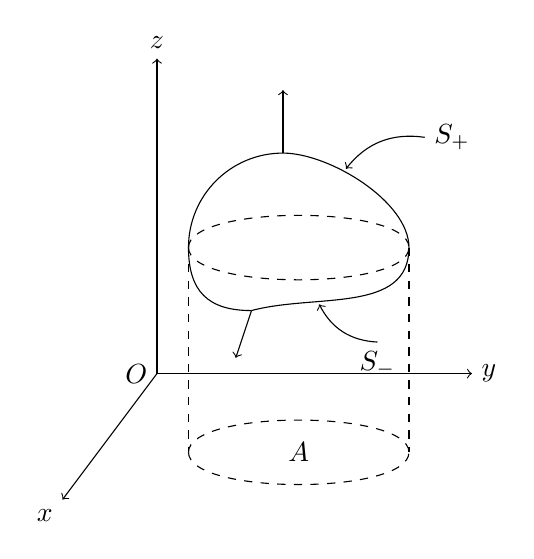
\begin{tikzpicture}[scale=0.8]
            \node (0) at (0, 0) {};
            \node [left] at (0) {$O$};
            \node (1) at (5, 0) {};
            \node [right] at (1) {$y$};
            \node (3) at (-1.5, -2) {};
            \node [below left] at (3) {$x$};
            \node (4) at (0, 5) {};
            \node [above] at (4) {$z$};
            \node (5) at (0.5, 2) {};
            \node (6) at (4, 2) {};
            \node (7) at (0.5, -1.25) {};
            \node (8) at (4, -1.25) {};
            \node (9) at (2, 3.5) {};
            \node (10) at (1.5, 1) {};
            \node (11) at (2, 4.5) {};
            \node [above] at (11) {$\bfn$};
            \node (12) at (1.25, 0.25) {};
            \node [right] at (12) {$\bfn$};
            \node (13) at (3, 3.25) {};
            \node (14) at (4.25, 3.75) {};` '
            \node [right] at (14) {$S_+$};
            \node (15) at (3.5, 0.5) {};
            \node [below] at (15) {$S_-$};
            \node (16) at (2.575, 1.1) {};
            \node (17) at (2.25, -1.25) {$A$};
            \draw [->] (0.center) to (4.center);
            \draw [->] (0.center) to (1.center);
            \draw [->] (0.center) to (3.center);
            \draw [in=180, out=90] (5.center) to (9.center);
            \draw [in=90, out=0, looseness=0.75] (9.center) to (6.center);
            \draw [in=-180, out=-90, looseness=1.25] (5.center) to (10.center);
            \draw [in=-90, out=15] (10.center) to (6.center);
            \draw [dashed, bend left=90, looseness=0.50] (5.center) to (6.center);
            \draw [dashed, bend right=90, looseness=0.50] (5.center) to (6.center);
            \draw [dashed, in=90, out=90, looseness=0.50] (7.center) to (8.center);
            \draw [dashed, bend right=90, looseness=0.50] (7.center) to (8.center);
            \draw [->] (9.center) to (11.center);
            \draw [->] (10.center) to (12.center);
            \draw [->, bend right] (14.center) to (13.center);
            \draw [->, bend right=330] (15.center) to (16.center);
            \draw [dashed] (5.center) to (7.center);
            \draw [dashed] (6.center) to (8.center);
        \end{tikzpicture}
    \end{center}
    Denote the upper and lower sides as 
    \[
        S_{\pm}=\left\{\mathbf{x}(x, y)=\begin{pmatrix}
            x \\
            y \\
            g_{\pm}(x, y)
        \end{pmatrix},(x, y) \in A\right\}.
    \]
    Then the volumn integral is 
    \begin{align*}
        \int_{V} \frac{\partial F_{z}}{\partial z} \mathrm{~d} V &=\iint_{A}\left[\int_{g_{-}(x, y)}^{g_{+}(x, y)} \frac{\partial F_{z}}{\partial z} \mathrm{~d} z\right] \mathrm{d} x \mathrm{~d} y \\
        &=\iint_{A}\left[F_{z}\left(x, y, g_{+}(x, y)\right)-F_{z}\left(x, y, g_{-}(x, y)\right)\right] \mathrm{d} x \mathrm{~d} y .\tag{$*$}
    \end{align*}
    On surfaces $ S_{\pm} $, we have 
    \[
        \mathrm{d} \mathbf{S}=\frac{\partial \mathbf{x}}{\partial x} \times \frac{\partial \mathbf{x}}{\partial y} \mathrm{~d} x \mathrm{~d} y=\begin{pmatrix}
            -\partial g_{\pm} / \partial x \\
            -\partial g_{\pm} / \partial y \\
            1 
        \end{pmatrix} \mathrm{d} x \mathrm{~d} y.
    \]
    By choosing suitable normals, we have
    \[
        \mathrm{d} \mathbf{S}=\pm\begin{pmatrix}
            -\partial g_{\pm} / \partial x \\
            -\partial g_{\pm} / \partial y \\
            1
        \end{pmatrix} \mathrm{d} x \mathrm{~d} y.
    \]
    Hence 
    \begin{align*}
        \int_{\partial V} F_{z} \mathbf{e}_{z} \cdot \mathrm{d} \mathbf{S} &=\left[\int_{S_{+}}+\int_{S_{-}}\right] F_{z} \mathbf{e}_{z} \cdot \mathrm{d} \mathbf{S} \\
        &=\iint_{A} F_{z}\left(x, y, g_{+}(x, y)\right) \mathrm{d} x \mathrm{~d} y-\iint_{A} F_{z}\left(x, y, g_{-}(x, y)\right) \mathrm{d} x \mathrm{~d} y \\
        &=\int_{V} \frac{\partial F_{z}}{\partial z} \mathrm{~d} V\quad \text{from ($*$)} .
    \end{align*}
    In exactly the same way, 
    \[
        \int_{V} \frac{\partial F_{x}}{\partial x} \mathrm{~d} V=\int_{\partial V} F_{x} \mathbf{e}_{x} \cdot \mathrm{d} \mathbf{S}, \quad \int_{V} \frac{\partial F_{y}}{\partial y} \mathrm{~d} V=\int_{\partial V} F_{y} \mathbf{e}_{y} \cdot \mathrm{d} \mathbf{S} .
    \]
    Summing up gives the result. The same method of proof holds for the two dimensional version of the divergence theorem. Our proof only holds for simple regions (e.g. convex), but can be modified so that it works on much more complex regions.
\end{proof}

We prove Green's theorem and Stokes' theorem by introducing 
\begin{proposition}
    Divergence theorem $ \Longrightarrow  $ Green's theorem.
\end{proposition}
\begin{proposition}
    Green's theorem $ \Longrightarrow  $ Stokes' theorem.
\end{proposition}
\begin{proof}[Proof of proposition 1.7]
    Use 2D divergence theorem on $ \bfF = (Q,-P) $, we get 
    \[
        \iint_{A} \left( \frac{\partial Q}{\partial x}-\frac{\partial P}{\partial y}   \right)\dd x\dd y = \int_{A} \div\bfF \,\mathrm{d}A  = \oint_{\partial A} \bfF \cdot \mathbf{n}\dd s.
    \]
    If $ \partial A $ is parametrised wrt arc-length, then unit tangent vector is given by $ \bft=(x'(s),y'(s)) $. Hence the normal vector must be $ \bfn = (y'(s),-x'(s)) $ (check). So 
    \[
        \bfF \cdot \mathbf{n} \dd s = Q \frac{\mathrm{d}y}{\mathrm{d}s}\dd s+ P \frac{\mathrm{d}x}{\mathrm{d}s}\dd s = P\dd x+Q\dd y,
    \]
    giving Green's theorem.
\end{proof}
\begin{proof}[Proof of proposition 1.8]
    Consider a regular surface 
    \[
        S = \{\bfx=\bfx(u,v): (u,v)\in A\}.
    \]
    Then the boundary is (see Analysis and Topology)
    \[
        \partial S = \{\bfx=\bfx(u,v): (u,v)\in \partial A\}.
    \]
    Green's theorem gives 
    \[
        \oint_{\partial A} P\dd u+Q\dd v = \iint_{A} \left( \frac{\partial Q}{\partial u}-\frac{\partial P}{\partial v}   \right)\dd u\dd v.
    \]
    Make choices 
    \[
        P(u,v) = \bfF(\bfx(u,v)) \cdot \frac{\partial \bfx}{\partial u},\quad Q(u,v) = \bfF(\bfx(u,v)) \cdot \frac{\partial \bfx}{\partial v}.  
    \]
    Then 
    \[
        P \mathrm{~d} u+Q \mathrm{~d} v=\mathbf{F}(\mathbf{x}(u, v)) \cdot\left(\frac{\partial \mathbf{x}}{\partial u} \mathrm{~d} u+\frac{\partial \mathbf{x}}{\partial v} \mathrm{~d} v\right)=\mathbf{F}(\mathbf{x}(u, v)) \cdot \mathrm{d} \mathbf{x}(u, v)
    \]
    which gives 
    \[
        \oint_{\partial A} P\dd u+Q\dd v = \oint_{\partial S} \bfF \cdot \rmd\bfx.
    \]
    For the other side of Stokes, 
    \[
        \frac{\partial Q}{\partial u}=\frac{\partial x_{j}}{\partial u} \frac{\partial F_{i}}{\partial x_{j}} \frac{\partial x_{i}}{\partial v}+F_{i} \frac{\partial^{2} x_{i}}{\partial u \partial v}\quad \frac{\partial P}{\partial v}=\frac{\partial x_{j}}{\partial v} \frac{\partial F_{i}}{\partial x_{j}} \frac{\partial x_{i}}{\partial u}+F_{i} \frac{\partial^{2} x_{i}}{\partial u \partial v}.
    \]
    This gives
    \begin{align*}
        \frac{\partial Q}{\partial u}-\frac{\partial P}{\partial v} &=\left(\frac{\partial x_{i}}{\partial v} \frac{\partial x_{j}}{\partial u}-\frac{\partial x_{i}}{\partial u} \frac{\partial x_{j}}{\partial v}\right) \frac{\partial F_{i}}{\partial x_{j}} \\
        &=\left(\delta_{i p} \delta_{j q}-\delta_{i q} \delta_{j p}\right) \frac{\partial F_{i}}{\partial x_{j}} \frac{\partial x_{p}}{\partial v} \frac{\partial x_{q}}{\partial u} \\
        &=\epsilon_{i j k} \epsilon_{p q k} \frac{\partial F_{i}}{\partial x_{j}} \frac{\partial x_{p}}{\partial v} \frac{\partial x_{q}}{\partial u} \\
        &=(\nabla \times \mathbf{F}) \cdot\left(\frac{\partial \mathbf{x}}{\partial u} \times \frac{\partial \mathbf{x}}{\partial v}\right)
    \end{align*}
    meaning that
    \[
        \iint_{A}\left(\frac{\partial Q}{\partial u}-\frac{\partial P}{\partial v}\right) \mathrm{d} u \mathrm{~d} v=\iint_{A}(\nabla \times \mathbf{F}) \cdot\left(\frac{\partial \mathbf{x}}{\partial u} \times \frac{\partial \mathbf{x}}{\partial v}\right) \mathrm{d} u \mathrm{~d} v=\int_{S}(\nabla \times \mathbf{F}) \cdot \mathrm{d} \mathbf{S} .
    \]
    So we have Stokes' theorem from Green's theorem. Note that this proof also works if the boundary of $A$ is a collection of disjoint curves.
\end{proof}